%% LyX 2.3.3 created this file.  For more info, see http://www.lyx.org/.
%% Do not edit unless you really know what you are doing.
\documentclass[12pt,english,sort&compress]{article}
\usepackage{mathpazo}
\usepackage[T1]{fontenc}
\usepackage[utf8]{inputenc}
\usepackage{geometry}
\geometry{verbose,tmargin=2cm,bmargin=2cm,lmargin=2cm,rmargin=2cm}
\setlength{\parskip}{\medskipamount}
\setlength{\parindent}{0pt}
\synctex=-1
\usepackage{babel}
\usepackage{units}
\usepackage{textcomp}
\usepackage{mathtools}
\usepackage{enumitem}
\usepackage{amsmath}
\usepackage{amssymb}
\usepackage{graphicx}
\usepackage[numbers]{natbib}
\usepackage[unicode=true,pdfusetitle,
 bookmarks=true,bookmarksnumbered=false,bookmarksopen=false,
 breaklinks=false,pdfborder={0 0 0},pdfborderstyle={},backref=false,colorlinks=false]
 {hyperref}

\makeatletter
%%%%%%%%%%%%%%%%%%%%%%%%%%%%%% Textclass specific LaTeX commands.
\newlength{\lyxlabelwidth}      % auxiliary length 
\newcommand{\lyxaddress}[1]{
	\par {\raggedright #1
	\vspace{1.4em}
	\noindent\par}
}

\@ifundefined{date}{}{\date{}}
%%%%%%%%%%%%%%%%%%%%%%%%%%%%%% User specified LaTeX commands.
\usepackage{fouriernc}
\usepackage{textcomp} % Needed for degC
\usepackage{kbordermatrix}
\usepackage{comment}

\usepackage{graphicx}
\newcommand\wlength{2.5em}
\newcommand\w[1]{\makebox[\wlength]{$#1$}}
\newcommand\minus[1]{\mathllap{-}#1}

\makeatother

\begin{document}
\title{Accelerating Reactive Transport Modeling:\\
On-Demand Learning Algorithm for Faster\\
Chemical Equilibrium Calculations}
\author{Allan M. M. Leal$^{\text{a,}}$\thanks{Corresponding author}\\
{\footnotesize{}\href{mailto:allan.leal@erdw.ethz.ch}{allan.leal@erdw.ethz.ch}}
\and Svetlana Kyas$^{\text{a}}$\\
{\footnotesize{}\href{mailto:svetlana.kyas@ethz.ch}{svetlana.kyas@ethz.ch}}
\and Dmitrii A. Kulik$^{\mathrm{b}}$\\
{\footnotesize{}\href{mailto:dmitrii.kulik@psi.ch}{dmitrii.kulik@psi.ch}}
\and Martin O. Saar$^{\text{a}}$\\
 {\footnotesize{}\href{mailto:msaar@ethz.ch}{msaar@ethz.ch}}}
\maketitle

\lyxaddress{\begin{center}
{\small{}$^{\text{a}}$}\emph{\small{}Institute of Geophysics, Department
of Earth Sciences, ETH Zürich, Switzerland\\[0.5em]}{\small{}$^{\text{b}}$}\emph{\small{}Laboratory
for Waste Management, Nuclear Energy and Safety Research Department,}{\small{}}\\
\emph{\small{}Paul Scherrer Institute, 5232 Villigen PSI, Switzerland}
\par\end{center}}
\begin{abstract}
During reactive transport modeling, the computational cost associated
with chemical reaction calculations is often 10–10'000 times higher
than that of transport calculations. Chemical equilibrium calculations
performed in every mesh cell and at every time step of the simulation
are often responsible for this high computing costs. We consider thus
an \emph{on-demand learning strategy} that enables chemical equilibrium
problems during a reactive transport simulation to be quickly and
accurately predicted using previously collected solution knowledge
of chemical equilibrium problems within the same simulation. We demonstrate
the use of this smart chemical equilibrium algorithm in a reactive
transport modeling example, in which a speedup of two orders of magnitude
is achieved. This algorithm has been implemented in Reaktoro, a unified
open-source framework for modeling chemically reactive systems.
\end{abstract}

\section{Introduction}

In reactive transport simulations, coupled chemical and physical processes
are modeled to understand phenomena that involve chemical reactions
and transport of chemical species. Examples of chemical processes
are reactions between species in an aqueous fluid leading to precipitation
of solid minerals, or their reaction with existing rock minerals causing
mineral dissolution. Examples of physical processes are the advection
of chemical species in a fluid that flows with a certain velocity,
or the diffusion of those fluid species as a result of the concentration
gradient across the medium. Because of the various processes considered
in a reactive transport model, the resulting computer simulations
are usually time-consuming.

Often, the relatively long computing time of reactive transport simulations
can be attributed to the need of performing millions to billions of
chemical reaction calculations. These are \emph{chemical kinetics}
and\slash or \emph{chemical equilibrium calculations} performed on
every mesh cell, at every time step of the simulation. These chemical
reaction calculations are computationally expensive because they involve
iterative algorithms to solve systems of non-linear algebraic and\slash or
differential equations \citep{Leal2017}. As a result, it triggers
repeated evaluations of thermodynamic properties, such as activity\slash fugacity
coefficients (sometimes using computationally demanding models such
as \citet{Pitzer1973} for aqueous phases and \citet{Peng1976} for
gaseous/liquid phases).

Thus, speeding up reactive transport modeling by a significant factor
may only be accomplished by first accelerating chemical reaction calculations
in general, and chemical equilibrium calculations in particular. The
latter is essential when employing a \emph{partial local chemical
equilibrium assumption} \citep{Ramshaw1980,Ramshaw1981,Ramshaw1985,Ramshaw1995,Lichtner1985,Steefel1994,Steefel1996}.
This assumes that species reacting at relatively high rates (e.g.,
aqueous, gaseous species) are under continual chemical equilibrium
at every point in space, whereas species reacting at slow to moderate
rates (e.g., mineral species) do so according to kinetic rate laws.
Thus, accelerating those millions to billions of chemical equilibrium
calculations over the course of massive numerical reactive transport
simulations is essential when using fine-resolution meshes, large
three-dimensional domains, and\slash or long simulation times at fine
temporal resolutions.

Major advances in developing fast, accurate, and robust methods for
chemical equilibrium calculations have been done for the past decades.
These are either based on the\emph{ Gibbs energy minimization} (GEM)
or the \emph{law of mass action} (LMA) formulations \citep{White1958,Smith1980,Smith1982,Alberty1992b,Crerar1975,DeCapitani1987,Eriksson1989,Ghiorso1994,Gordon1971,Gordon1994a,Gordon1996,Harvey2013,Harvie1987,Karpov1997,Karpov2001,Karpov2002,Koukkari2011a,Kulik2013,Leal2013,Leal2014,Leal2016a,Leal2016c,Leal2017,Morel1972,Neron2012,Nordstrom1979,Trangenstein1986,VanZeggeren1970,Vonka1995,Wolery1975,Zeleznik1960}.
However, even if one could devise a hypothetical algorithm that would
always converge in a single iteration, instead of the typical few
to dozens of iterations, the computational cost of chemical equilibrium
calculations could still be dominant in a reactive transport simulation.
This is because, in this single iteration, we would still need to
evaluate expensive thermodynamic models and solve a matrix equation
when using a Newton-based GEM or LMA algorithm. A substantial acceleration
of these simulations can thus be achieved if these costly operations
can be bypassed whenever possible\emph{.}

During a time step of a reactive transport simulation, chemical equilibrium
calculations are needed in all mesh cells. Often, many of these calculations
are similar to previously performed ones, either within the same time-step
and\slash or mesh cell or at different points in space and\slash or
time. We say two chemical equilibrium problems are similar when their
input conditions are sufficiently close (i.e., similar temperature,
pressure, amounts of chemical elements and electric charge of each
phase containing electrically charged species \citep{Smith1982}).
These chemical equilibrium calculations are hardly identical so that
we can not simply assume a previously computed result as the exact
result of the new calculation. Interpolating is also not an appropriate
approach because it can violate mass conservation of elements (i.e.,
there is a deviation between the input element amounts and the amounts
of elements calculated from the interpolated species amounts).

The principle of the \emph{smart chemical equilibrium algorithm} discussed
here is exactly to \emph{avoid} as much as possible full and expensive
chemical equilibrium calculations during the reactive transport simulation.
By using \emph{sensitivity derivatives} of previously computed equilibrium
states, we can quickly and accurately estimate the new equilibrium
state at similar input conditions. These derivatives tell us how sensitive
the computed species amounts at a certain equilibrium state are with
respect to infinitesimal changes in temperature, pressure, and element
amounts. Thus, multiplying these sensitivity derivatives by respective
differences in input conditions (e.g., differences in temperature
or the amount of a particular element), we can estimate the variation
in the output. For example, we can estimate how much the species amounts
would change by increasing temperature by 1~°C, by adding 1~mmol
of HCl into the system (which is equivalent to adding 1~mmol of elements
H and Cl), or by combining these with other input changes. We remark
that the use of sensitive derivatives to estimate the solution of
an equilibrium problem is inherently \emph{mass conservative}. This
is because these derivatives are computed by deriving the chemical
equilibrium equations, which include the equations of element mass
conservation.


\subsubsection*{Related Work}

Increasing the speed of chemical reaction calculations, i.e., equilibrium
and\slash or kinetics, is an active research topic. The majority of
the existing methodologies are based on the use of \emph{surrogate
models} and\slash or \emph{machine learning} schemes, which use a
computationally cheaper model (e.g., linearization, parameterization,
neural network) to approximate a complex nonlinear behavior.

In combustion chemistry, the pioneering work of \citet{Pope1997},
in speeding up \emph{chemical kinetics calculations, }considers approximations
of chemical kinetics paths using multiple linear regressions using
\emph{unstructured adaptive} \emph{storage/extraction technique} along
the simulation process. This approach is referred to in the literature
as \emph{in situ adaptive tabulation} (ISAT)\emph{ }algorithm\emph{.
}The ISAT approximation idea was later extended to \emph{nonlinear
model predictive control} (NMPC) in \citep{HedengrenEdgar2008}. ISAT
can be regarded as an alternative to artificial neural networks since
it does not require any preliminary training to simulate the behavior
of the model. Instead, it rearranges the model by new data trainings
\emph{on the fly} as simulations proceed. It also relies on the nearest
neighbor search algorithms, and an enhanced binary-tree retrieval
algorithm was investigated in \citep{Chen2018}. The ISAT algorithm
scales quadratically with increased dimension, approximates functions
with discontinuities, and provides explicit bounds on approximation
error. A series of parallel chemistry acceleration algorithms for
simulation of unsteady, compressible, reactive flows based on ISAT
technique was proposed in \citet{WuDongLi2018}.

In addition to the ISAT approach, several alternative storage-based
approaches have been suggested in the past for speeding up chemical
kinetics, including polynomial fits by \citet{Turanyi1994}, artificial
neural networks (see, e.g., \citet{ChristoMasriNebot1996,Blascoetall1998}),
and piece-wise reusable implementation of solution mapping (PRISM)
by \citet{TonseMoriartyBrownFrenklach2013}. The general property
of these approaches is the a priori creation of the approximation
model (whether it is skeleton model or neural network), which requires
extra effort usually but then evaluating a simplified model to speed
up the subsequent calculations. The PRISM method is similar to the
in situ approach, except that the stored data entries are not output
values and corresponding sensitivity derivatives, but the set of polynomials
covering a region of chemical composition space. The recorder speedup
for above-mentioned methods is about to 10-60.

The work of \citet{Jatnieks2016}, on the use of a surrogate model
for fast speciation calculations, is another initiative to accelerate
chemical equilibrium calculations in reactive transport modeling.
The construction of this surrogate model required a training stage
in advance, during which many random input conditions were used in
a speciation solver, PHREEQC \citep{Parkhurst2013}, and the resultant
outputs collected for statistical learning. During their numerical
experiment, 32 different statistical and machine learning methods
were tried to identify the potentially best one. For a specific reactive
transport modeling problem, \citet{Jatnieks2016} collected all possible
input-output combinations in speciation calculations, and from these,
7880 input-output samples (representing 80\% of the total known input-output
relationships) were used for training the statistical model. The various
constructed surrogate models were subsequently used in the reactive
transport simulation. Because these surrogate models relied on statistical
methods, mass conservation was often not accurate in their machine
learning estimates (i.e., the amounts of chemical elements in the
estimated-output species amounts did not correspond accurately to
the values given in the input).

The \emph{on-demand machine learning approach} used here has advantages
over conventional statistics-based machine learning methods. First,
the use of \emph{sensitivity derivatives} of the calculated equilibrium
states results in a method that better understands the behavior of
chemical systems on how it should react to the following changes in
the input equilibrium conditions. Secondly, the use of these sensitivity
derivatives permits extrapolating and predicting new equilibrium states
with much \emph{higher accuracy and confidence}. Thirdly, it requires
\emph{no a priori statistical training} before it can be applied in
a reactive transport simulation. Its on-demand learning characteristics
allow it to learn spontaneously only what is needed during a reactive
transport simulation to keep the predictions accurate enough. Note
that, when using a conventional approach, these computations are needed
anyway. Furthermore, this on-demand learning strategy is not only
simpler from an end-user point of view, but also potentially faster,
as it will save in general fewer input conditions compared to any
statistical approach that can only get more accurate the more it knows
in advance. Finally, the smart chemical equilibrium algorithm produces
outputs that \emph{always satisfy conservation conditions} of chemical
elements and electric charge, since these constraints are incorporated
into the calculation of the sensitivity derivatives (see \citet{Leal2017}).
This particularly distinguishes the discussed method from statistically-based
machine learning methods, which can fail in this aspect.


\subsubsection*{Organization}

This communication is organized as follows:
\begin{description}
\item [{Section~\ref{sec:Definitions-and-Notation}}] introduces definitions
and notation needed to describe the algorithm.
\item [{Section~\ref{sec:Method}}] formulates the smart chemical equilibrium
algorithm with details of the learning and prediction operations.
\item [{Section~\ref{sec:Results}}] demonstrates the performance and
accuracy of a reactive transport simulation using smart equilibrium
algorithm.
\item [{Section~\ref{sec:Discussion-and-Conclusions}}] discusses implications
and conclusions of this study together with a planned road-map for
further research efforts in this direction.
\end{description}

\section{Definitions and Notation\label{sec:Definitions-and-Notation}}

Considered throughout the paper, a \emph{chemical system} is a collection
of \emph{chemical species} composed of one or more \emph{elements}
and distributed among one or more \emph{phases}. The species can be
substances such as aqueous ions (e.g., Na$^{+}$(aq), Cl$^{-}$(aq),
HCO$_{3}^{-}$(aq)), neutral aqueous species (e.g., SiO2(aq), CO$_{2}$(aq),
H$_{2}$O(l)), gases (e.g., CO$_{2}$(g), CH$_{4}$(g), N$_{2}$(g)),
pure condensed phases (e.g., CaCO$_{3}$(s, calcite), SiO$_{2}$(s,
quartz), Al$_{2}$Si$_{2}$O$_{5}$(OH)$_{4}$(s, kaolinite)). Each
phase (e.g., aqueous, gaseous, liquid, solid solutions, a pure mineral,
plasma, etc.) is composed of one or more different chemical species
with homogeneous properties within their boundaries. The elements
are \emph{chemical elements }(e.g., H, O, C, Na, Cl, Ca, Si) and \emph{electrical
charge} (Z), but it can also be a linear combination of these, commonly
known as \emph{primary species} (e.g., H$^{+}$(aq), H$_{2}$O(l),
CO$_{2}$(aq)).

A chemical system can exist at infinitely many \emph{chemical states}.
A chemical state is defined here as the triplet $(T,P,n)$, where
$T$ is temperature, $P$ is pressure, and $n=(n_{1},\ldots,n_{\mathrm{N}})\in\mathbb{R}^{\text{N}}$
is the vector of species amounts, with $n_{i}$ denoting the amount
of the $i$th species and N the number of species. The vector of element
amounts $b=(b_{1},\ldots,b_{\mathrm{E}})\in\mathbb{R}^{\text{E}}$,
with $b_{j}$ being the amount of the $j$th element and $\text{E}$
the number of elements, is related to $n$ via the following mass
conservation equation:
\begin{equation}
An=b,\label{eq:mass-balance}
\end{equation}
where $A$ is the \emph{formula matrix }of the chemical system \citep{Smith1982}
(whose dimensions are $\mathrm{E}\times\mathrm{N}$), with $A_{ji}$
denoting the coefficient of the $j$th element in the $i$th species.

\section{Method\label{sec:Method}}

Let a chemical equilibrium calculation be represented by the following
function:
\begin{equation}
n=\varphi(T,P,b),\label{eq:equilibrium-func}
\end{equation}
where $\varphi$ is an abstraction of the operations needed to solve
the fundamental Gibbs energy minimization problem:
\begin{equation}
\min_{n}G(T,P,n)\quad\text{subject to}\quad\left\{ \begin{aligned}An=b\\
n\geq0
\end{aligned}
\right.,\label{eq:gem-problem}
\end{equation}
at a prescribed temperature $T$, pressure $P$, and element amounts
$b=(b_{1},\ldots,b_{\mathrm{E}})$. In this problem, one aims to find
$n=(n_{1},\ldots,n_{\mathrm{N}})$ that minimizes the Gibbs energy
function of the system: 
\begin{equation}
G=\sum_{i=1}^{\text{N}}\mu_{i}n_{i},
\end{equation}
subject to the elemental mass conservation constraint equations $An=b$
and the non-negativity constraints for the species amounts, $n_{i}\geq0$.
The \emph{chemical potential} of the $i$th species $\mu_{i}=\mu_{i}(T,P,n)$
is defined as:
\begin{equation}
\mu_{i}=\mu_{i}^{\circ}+RT\ln a_{i},
\end{equation}
with $R$ denoting the universal gas constant, $\mu_{i}^{\circ}=\mu_{i}^{\circ}(T,P)$
the \emph{standard chemical potential} of the $i$th species, and
$a_{i}=a_{i}(T,P,n)$ the \emph{activity} of the $i$th species. Methods
for solving chemical equilibrium problem using either the Gibbs energy
minimization (GEM) or the law of mass action (LMA) methods are addressed
in Appendix~\ref{subsec:Chemical-equilibrium-equations} or with
more detail in \citet{Leal2016a,Leal2016c,Leal2017} and references
therein.

\subsection{First-Order Taylor Approximation\label{subsec:First-order-Taylor-approximation}}

Assume a chemical equilibrium calculation has been performed previously
with input conditions $(T^{\star},P^{\star},b^{\star})$, and a new
one needs to be performed with $(T,P,b)$ instead. Rather than computing
$n=\varphi(T,P,b)$, using the computationally expensive equilibrium
function $\varphi$ (cf. \ref{eq:equilibrium-func}), we first try
estimating $\bar{n}=(\bar{n}_{1},\ldots,\bar{n}_{\mathrm{N}})$ with
a \emph{first-order Taylor approximation}:
\begin{equation}
\bar{n}=n^{\star}+\frac{\partial\varphi}{\partial T}^{\star}(T-T^{\star})+\frac{\partial\varphi}{\partial P}^{\star}(P-P^{\star})+\frac{\partial\varphi}{\partial b}^{\star}(b-b^{\star}),\label{eq:smart-estimate}
\end{equation}
where $(\partial\varphi/\partial T)^{\star}$, $(\partial\varphi/\partial P)^{\star}$,
and $(\partial\varphi/\partial b)^{\star}$ are \emph{sensitivity
derivatives} of the reference chemical equilibrium state, which can
be equivalently written as $(\partial n/\partial T)^{\star}$, $(\partial n/\partial P)^{\star}$,
and $(\partial n/\partial b)^{\star}$, respectively. These sensitivity
derivatives permit us to estimate how the species amounts in an equilibrium
state change when small perturbations are applied to temperature,
pressure, and\slash or amounts of elements. By using them, we can
therefore quickly and accurately estimate entirely new states in the
vicinity of some previous and fully calculated chemical equilibrium
state.

\subsection{Nearest Neighbor Search\label{subsec:Nearest-Neighbor-Search}}

Let $\mathcal{I}$ represent the set of input conditions for the chemical
equilibrium problems that have been fully solved (i.e., using the
chemical equilibrium function $\varphi$):
\begin{equation}
\mathcal{I}=\left\{ (T^{k},P^{k},b^{k})\right\} _{k=1}^{\text{K}}.
\end{equation}
Furthermore, let $d^{k}$ denote the Euclidean distance from $(T^{k},P^{k},b^{k})$,
the input condition of the $k$th fully solved problem, to $(T,P,b)$,
the given input condition for the new equilibrium calculation:
\begin{equation}
d^{k}=\left[\left(T-T^{k}\right)^{2}+\left(P-P^{k}\right)^{2}+\sum_{j=1}^{\text{E}}\left(b_{j}-b_{j}^{k}\right)^{2}\right]^{\frac{1}{2}}\qquad k=1,\ldots,\mathrm{K}.
\end{equation}

For the first-order Taylor approximation presented before (Eq.~\ref{eq:smart-estimate}),
a potentially suitable candidate for $(T^{\star},P^{\star},b^{\star})$
is the \emph{nearest neighbor} of $(T,P,b)$ among all inputs in $\mathcal{I}$
(i.e., the saved input with the shortest Euclidean distance to $(T,P,b)$).
Note that the other norms can be used to define distance, although
we obtained convincing results with Euclidean norm.

There are plenty of algorithms for the fast multi-dimensional nearest
neighbor search operations in the literature. The use of \emph{kd-tree
data structures} to store the inputs, for example, may permit us to
obtain an algorithm complexity $\log_{2}(\mathrm{K})$, where $\mathrm{K}$
is the number of entries in the set. This implies that in a set with
1024 entries, only about 10 distance comparisons are done. This contrasts
with a linear search algorithm, with complexity $O(\mathrm{K})$,
which would thus require instead 1024 corresponding evaluations and
comparisons.

These algorithms, however, may behave very differently depending on
the number and dimension of the input vectors collected. Tree data
structures have a more sparse memory pattern than contiguous memory
data structures, such as arrays\slash vectors. The portions of the
data for the latter can be cached by the CPU, permitting thus their
processing at much faster rates. This implies that for sufficiently
small data-sets (e.g, with dozens to perhaps a few hundred entries),
tree-based search algorithms could be sub-optimal. Under these circumstances,
a linear search algorithm, conjugated with contiguous memory data
structures, can be more efficient.

A combination of tree-based and linear search algorithms is then needed.
We can start with a linear search approach since initially there are
not many saved inputs of learned chemical equilibrium problems. Once
a certain number of inputs have been saved, we construct a kd-tree.
This will permit the construction of a more well-balanced kd-tree
(i.e., a tree whose sibling branches have similar number of entries),
and thus ensure faster search operations close to $\log_{2}(K)$ complexity.

In this proof-of-concept work, we have relied solely on a linear search
algorithm, which worked well in the acceleration of the reactive transport
problem shown later in Section~\ref{sec:Results}. Complementing
the computer implementation of the smart chemical equilibrium algorithm
with kd-tree search algorithms is an ongoing work.

\subsection{Acceptance Test}

\begin{figure}
\begin{centering}
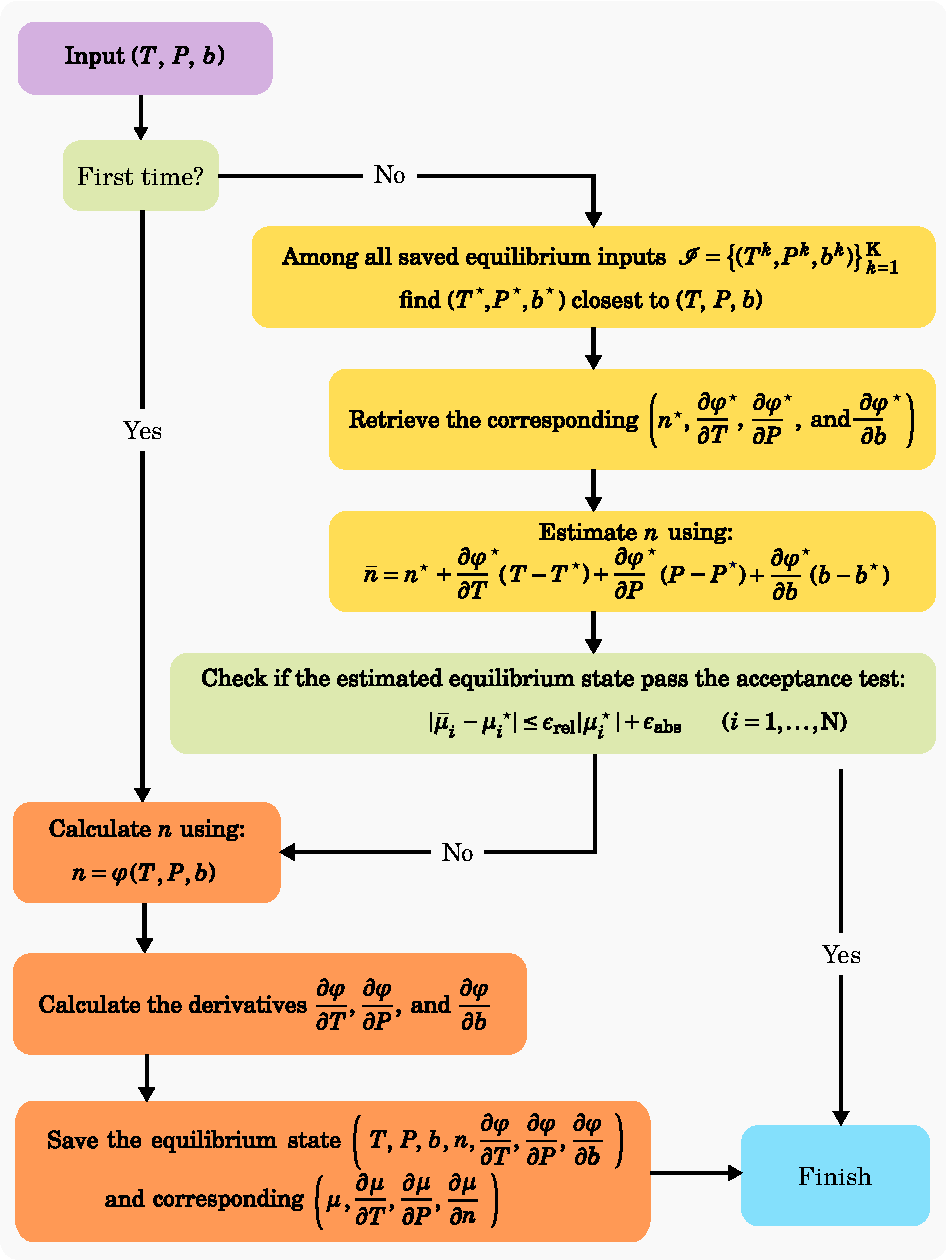
\includegraphics{figures/algorithm-flowchart-with-star}
\par\end{centering}
\caption{\label{fig:algorithm-diagram}Diagram of the smart chemical reaction
algorithm.}
\end{figure}

Once a predicted chemical equilibrium state is calculated, it must
be tested for acceptance. Due to the usage of the first-order Taylor
approximation, we need to ensure that the new estimated chemical equilibrium
state is not ``too far'' from the previous fully-calculated equilibrium
state used as a reference point. This could be done naively by checking
how much the species amounts changed from one state to another, using
the following test condition for all species:
\begin{equation}
|\bar{n}_{i}-n_{i}^{\star}|\leq\epsilon_{\text{rel}}|n_{i}^{\star}|+\epsilon_{\text{abs}}\qquad(i=1,\ldots,\text{N}).\label{eq:eq:acceptance-test-n}
\end{equation}
It controls how much the absolute and relative changes in the new
estimated species amounts $\bar{n}_{i}$ can be tolerated for given
absolute and relative tolerance parameters $\epsilon_{\text{abs}}$
and $\epsilon_{\text{rel}}$, respectively.

The major drawback of the tolerance test in Eq.~(\ref{eq:eq:acceptance-test-n})
is that it does not reflect the thermodynamic \emph{behavior of stable
phases}. Consider, for instance, a chemical system with two stable
phases: an aqueous solution saturated with a mineral. Adding more
of that mineral to the system will not alter the composition of the
fluid, but just increase its current solid amount. In such conditions,
the acceptance test based on species amounts would fail even though
the estimated chemical equilibrium state using first-order sensitivity
derivatives would be exact. This happens due to linear growth of the
amount of mineral while the amount of each aqueous species would remain
constant.

For the example above, assuming the perturbation of the system is
made only via the addition of the mineral, without changes in temperature
and pressure, there is one thermodynamic quantity that would remain
constant: $\mu_{i}$, the chemical potentials of the mineral species.
This behavior has inspired us to use chemical potentials in the acceptance
test: 
\begin{equation}
|\bar{\mu}_{i}-\mu_{i}^{\star}|\leq\epsilon_{\text{rel}}|\mu_{i}^{\star}|+\epsilon_{\text{abs}}\qquad(i=1,\ldots,\text{N}),\label{eq:acceptance-test-mu}
\end{equation}
where $\bar{\mu}_{i}$ is the estimated chemical potential of the
$i$th species at the new chemical equilibrium state: 
\begin{equation}
\bar{\mu}=\mu^{\star}+\frac{\partial\mu}{\partial T}^{\star}(T-T^{\star})+\frac{\partial\mu}{\partial P}^{\star}(P-P^{\star})+\frac{\partial\mu}{\partial n}^{\star}(n-n^{\star}),\label{eq:mu-estimated}
\end{equation}
where $(\partial\mu/\partial T)^{\star}\in\mathbb{R}^{\text{N}}$,
$(\partial\mu/\partial P)^{\star}\in\mathbb{R}^{\text{N}}$, and $(\partial\mu/\partial n)^{\star}\in\mathbb{R}^{\text{N\ensuremath{\times}N}}$
are chemical potential sensitivities evaluated at the equilibrium
state with input conditions $(T^{\star},P^{\star},b^{\star})$. 

\textbf{Remark:} For the law of mass-action (LMA) methods, in which
no access to standard chemical potentials exists in some cases (e.g.,
the thermodynamic database used only contains equilibrium constants
of reactions), a similar, but \emph{not equivalent}, test exploits
activities:
\begin{equation}
|\ln\bar{a}_{i}-\ln a_{i}^{\star}|\leq\epsilon_{\text{rel}}|\ln a_{i}^{\star}|+\epsilon_{\text{abs}}\qquad(i=1,\ldots,\text{N}).\label{eq:acceptance-test-lna}
\end{equation}
Note, however, that activities are in general less sensitive to temperature
variations than standard chemical potentials, and thus the above alternative
acceptance test would be less complete than equation~(\ref{eq:acceptance-test-mu})
and more indifferent towards temperature changes. To fix this, one
could use the approach detailed in \citet{Leal2016b} that permits
apparent standard chemical potentials of the species to be calculated
using equilibrium constants of reactions.

\subsection{Smart Chemical Equilibrium Algorithm \label{subsec:Smart-chemical-equilibrium}}

The smart chemical equilibrium algorithm applied here is capable of
remembering past calculations and making use of them to quickly and
accurately estimate new equilibrium states. The flowchart in Figure~\ref{fig:algorithm-diagram}
illustrates the main steps of the algorithm. In its first chemical
equilibrium calculation with given $(T,P,b)$ conditions, it solves
the Gibbs energy minimization problem (Eq.~\ref{eq:gem-problem}).
This is represented in Figure~\ref{fig:algorithm-diagram} using
the computationally expensive equilibrium function~$\varphi$ (Eq.~\ref{eq:equilibrium-func}).
Once this is done, we need to save the following information for the
future computations. This will enable making fast and accurate predictions
of equilibrium states whose input conditions are relatively close
to the one just recorded:
\begin{itemize}
\item the input conditions $(T,P,b)$;
\item the corresponding calculated equilibrium amounts of species $n$;
\item the sensitivity derivatives of the calculated equilibrium state: $\partial\varphi/\partial T$,
$\partial\varphi/\partial P$, and $\partial\varphi/\partial b$;
and
\item the derivatives of the chemical potentials $\partial\mu/\partial T$,
$\partial\mu/\partial P$, and $\partial\mu/\partial n$.
\end{itemize}
See \citet{Leal2017} for a description of how to accurately calculate
these sensitivities and thermodynamic property derivatives.

Next time the algorithm is asked to solve a new equilibrium problem,
it first does so by searching for the closest $(T^{\star},P^{\star},b^{\star})$
to the given $(T,P,b)$ among all saved equilibrium input conditions
in $\mathcal{I}$ . Once the search is concluded, the previously calculated
potentially suitable equilibrium state is used to estimate the new
equilibrium state using equation~(\ref{eq:smart-estimate}).

Finally, it remains to check if the estimated equilibrium state is
accurate enough using the acceptance test defined by Eq.~(\ref{eq:acceptance-test-mu}).
If the test succeeds, then the equilibrium calculation ends. Otherwise,
a complete chemical equilibrium calculation at $(T,P,b)$ is performed
using $n=\varphi(T,P,b)$ followed by similar derivative evaluation
operations as presented above when the smart equilibrium algorithm
is invoked the first time.


\section{Results\label{sec:Results}}

We present the use of the smart chemical equilibrium algorithm in
reactive transport simulation, and show how its performance compares
to the use of a conventional chemical equilibrium algorithm based
on the Gibbs energy minimization \citep{Leal2016a,Leal2017}. For
details on how we solve the reactive transport equations, see Appendix~\ref{sec:Reactive-Transport-Equations}.

\subsection{Reactive Transport Problem\label{subsec:Reactive-Transport-Problem}}

We illustrate the reactive transport modeling example carried out
in this work in Figure~\ref{fig:illustration-reactive-transport-model}.
In this figure, we show the initial mineral composition of a porous
rock core: 98\%$_{\text{vol}}$ SiO$_{2}$(quartz) and 2\%$_{\text{vol}}$
CaCO$_{3}$(calcite) with an initial porosity of 10\%. The resident
fluid is a 0.70 molal NaCl brine in equilibrium with the rock minerals
(our calculated equilibrium state indicates a pH of about 9.2). The
aqueous fluid injected on the left side of this rock core is the result
of mixing 1 kg of water with 0.90 moles of NaCl, 0.05 moles of MgCl$_{2}$,
0.01 moles of CaCl$_{2}$, and 0.75 moles of CO$_{2}$. This amount
of CO$_{2}$ is enough to bring the aqueous fluid close to CO$_{2}$
saturation, and thus in an acidic state, with a calculated pH of 3.05.
The temperature and pressure of both resident and injected fluids
are 60~°C and 100~bar, respectively. The reactive transport modeling
assumes a constant fluid velocity of $v=\unit[1]{m/week}$ ($\unit[5.95\cdot10^{-6}]{m/s}$)
and the same diffusion coefficient $D=\unit[10^{-9}]{m^{2}/s}$ for
all fluid species, without dispersivity. Our intention in this proof-of-concept
paper is to demonstrate the potential of the on-demand learning algorithm,
which will be followed by more advanced demonstrations in future work
(e.g., more heterogeneous media, three-dimensional meshes, etc.).

\begin{figure}
\begin{centering}
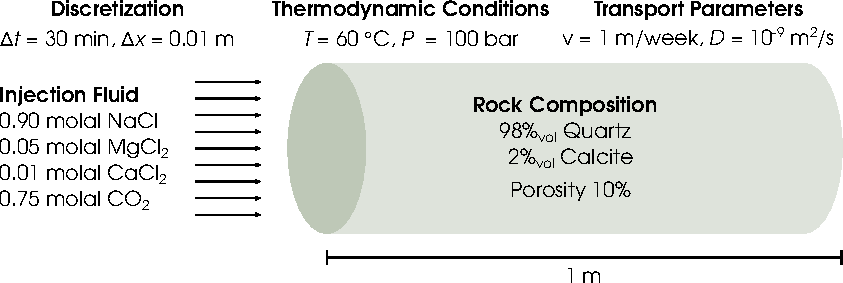
\includegraphics[width=1\textwidth]{figures/transport-scheme}
\par\end{centering}
\caption{\label{fig:illustration-reactive-transport-model}Illustration of
the reactive transport modeling along a one dimensional rock core
with details of the injection fluid and rock composition, transport
parameters, and numerical discretization.}
\end{figure}

The activity coefficients of the aqueous species are calculated using
the Pitzer model \citep{Pitzer1973} formulated by \citet{Harvie1984},
except for the aqueous species CO$_{2}$(aq), for which the \citet{drummond1981boiling}
model is applied. The standard chemical potentials of the species
are calculated using the equations of state of \citet{Helgeson1974,Helgeson1978,Tanger1988,Shock1988}
and \citet{Shock1992}. The database file \texttt{slop98.dat,} from
the software SUPCRT92 \citep{Johnson1992}, is used to obtain corresponding
parameters. The equation of state of \citet{Wagner2002} is chosen
to compute the density of water and its temperature and pressure derivatives.
These assumptions yield the system of 36 chemical species with 9 elements.
Although it could be considered in principle, dissolution and precipitation
kinetics of both calcite and dolomite minerals are neglected in this
particular example (i.e., the local equilibrium assumption is employed).
In such a way, we can assess how accurate the smart chemical equilibrium
predictions are when phase transitions happen (e.g., when calcite
fully dissolves, and when dolomite starts precipitation). We remark,
however, that the extension of the on-demand learning algorithm for
accelerating chemical kinetics calculations is already an on-going
work. 

\begin{figure}
\begin{centering}
\begin{minipage}[t]{0.5\columnwidth}%
\begin{center}
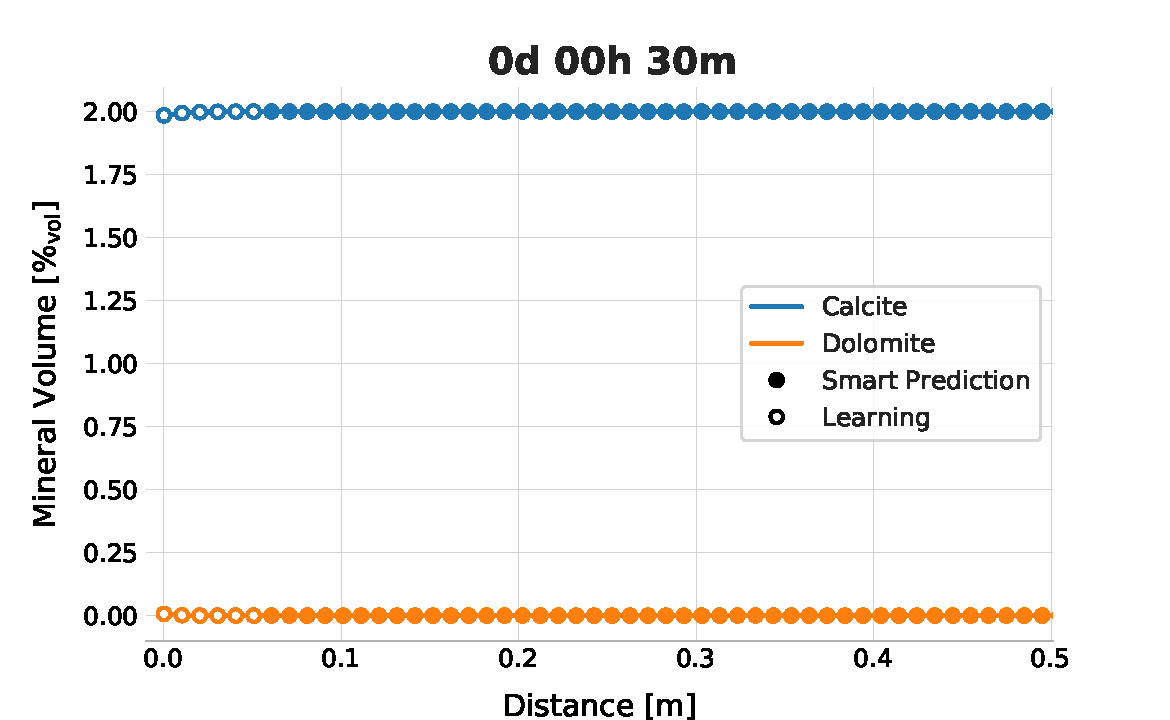
\includegraphics[width=1\textwidth]{figures/calcite-dolomite-1}
\par\end{center}
\begin{center}
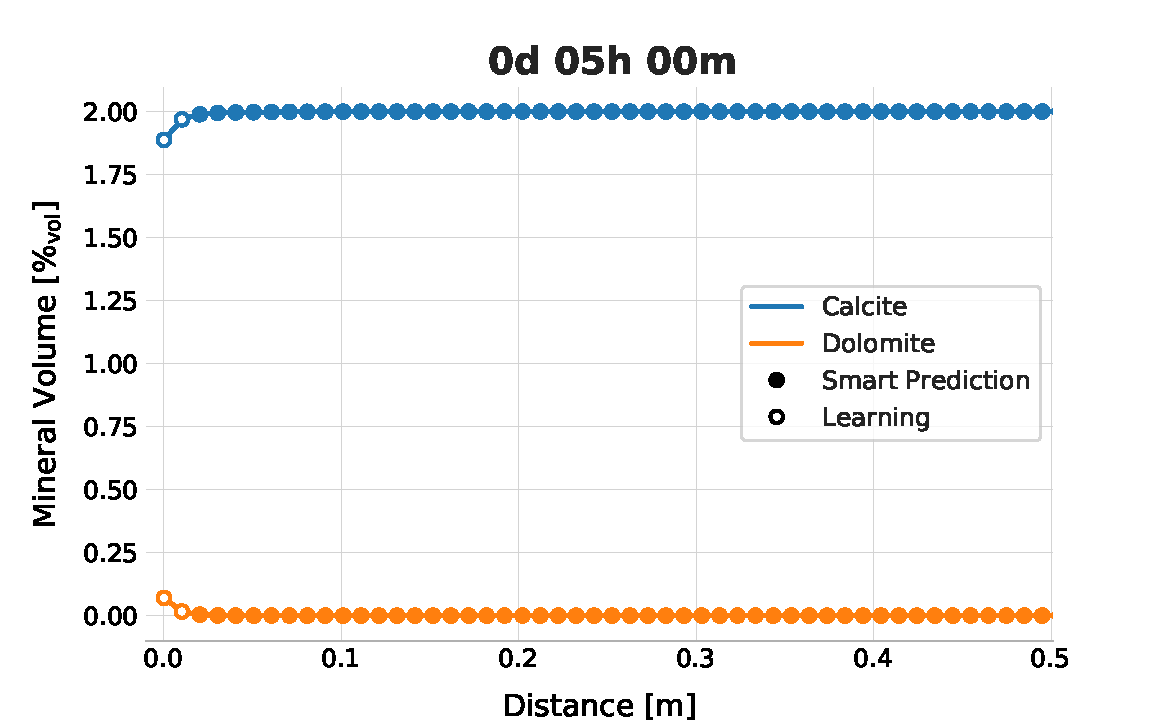
\includegraphics[width=1\textwidth]{figures/calcite-dolomite-10}
\par\end{center}
\begin{center}
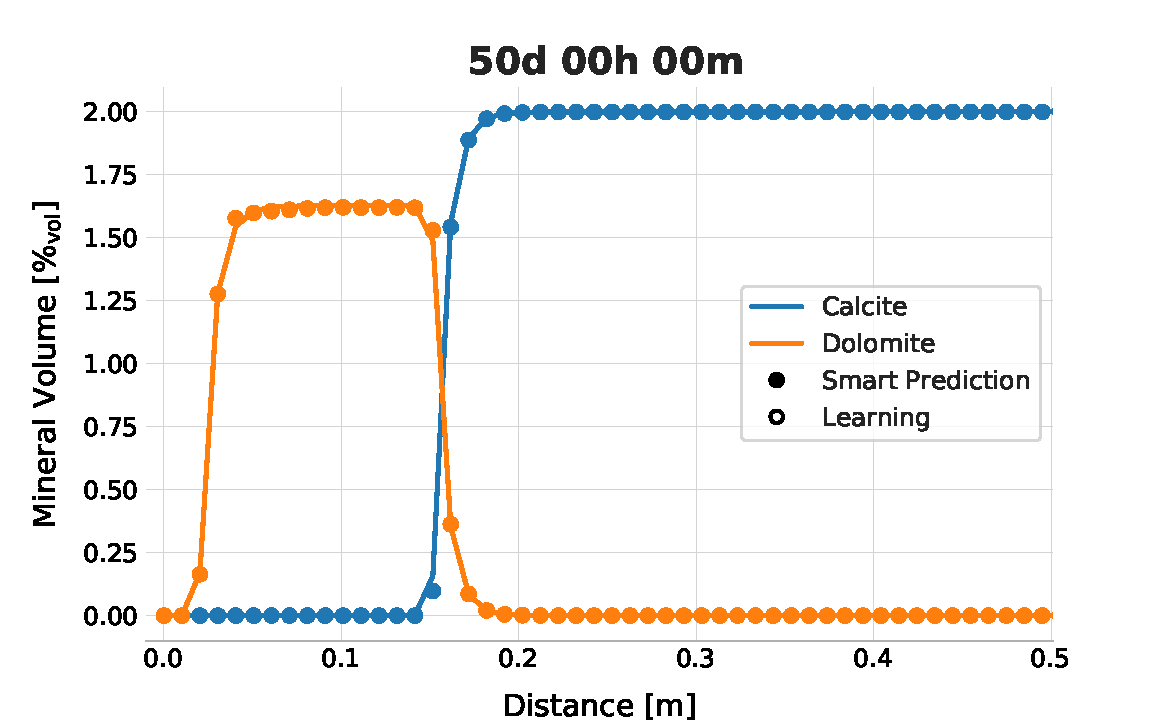
\includegraphics[width=1\textwidth]{figures/calcite-dolomite-2400}
\par\end{center}%
\end{minipage}%
\begin{minipage}[t]{0.5\columnwidth}%
\begin{center}
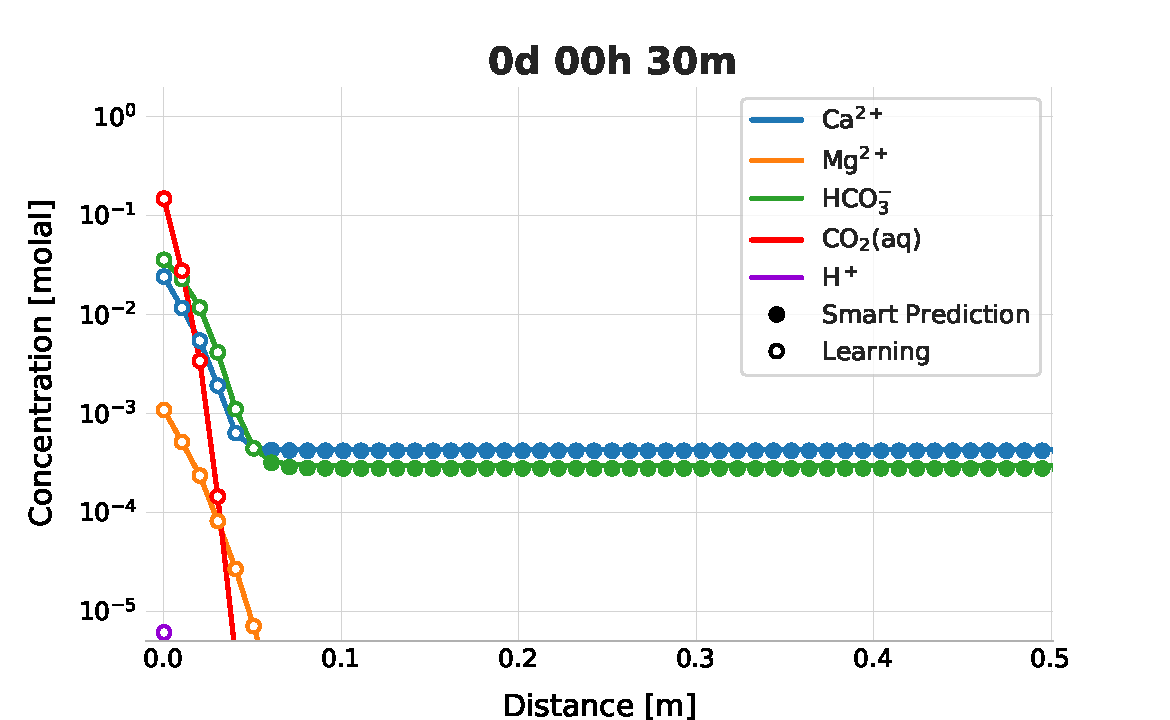
\includegraphics[width=1\textwidth]{figures/aqueous-species-1}
\par\end{center}
\begin{center}
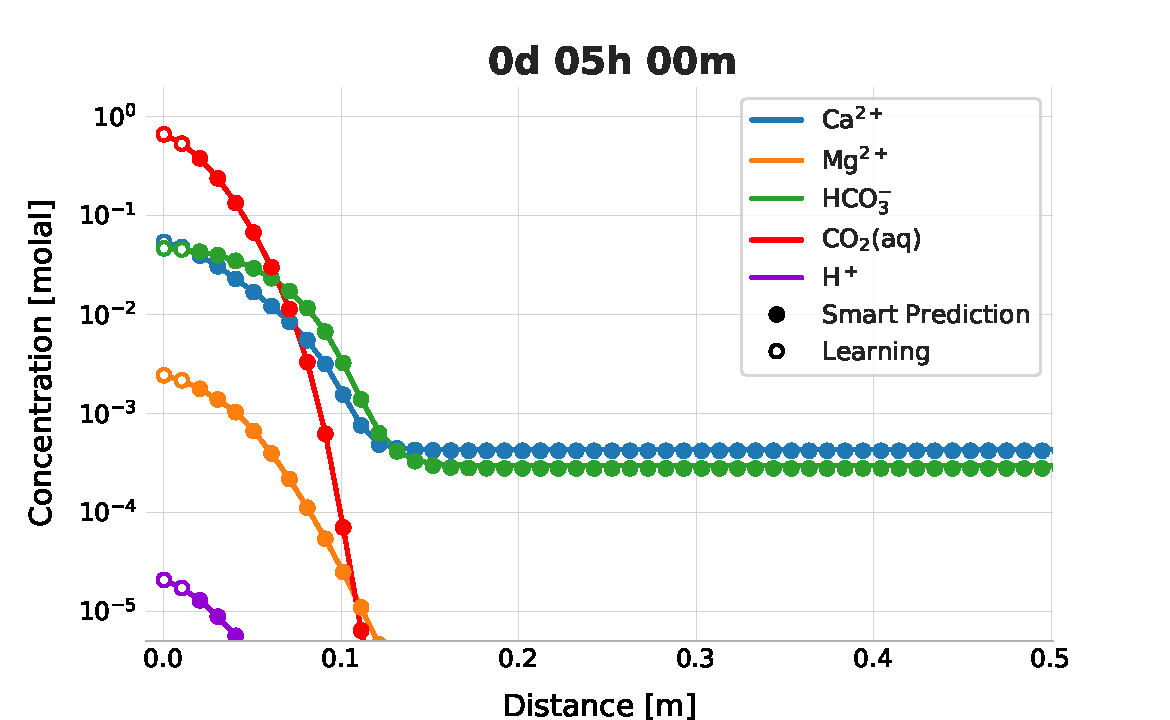
\includegraphics[width=1\textwidth]{figures/aqueous-species-10}
\par\end{center}
\begin{center}
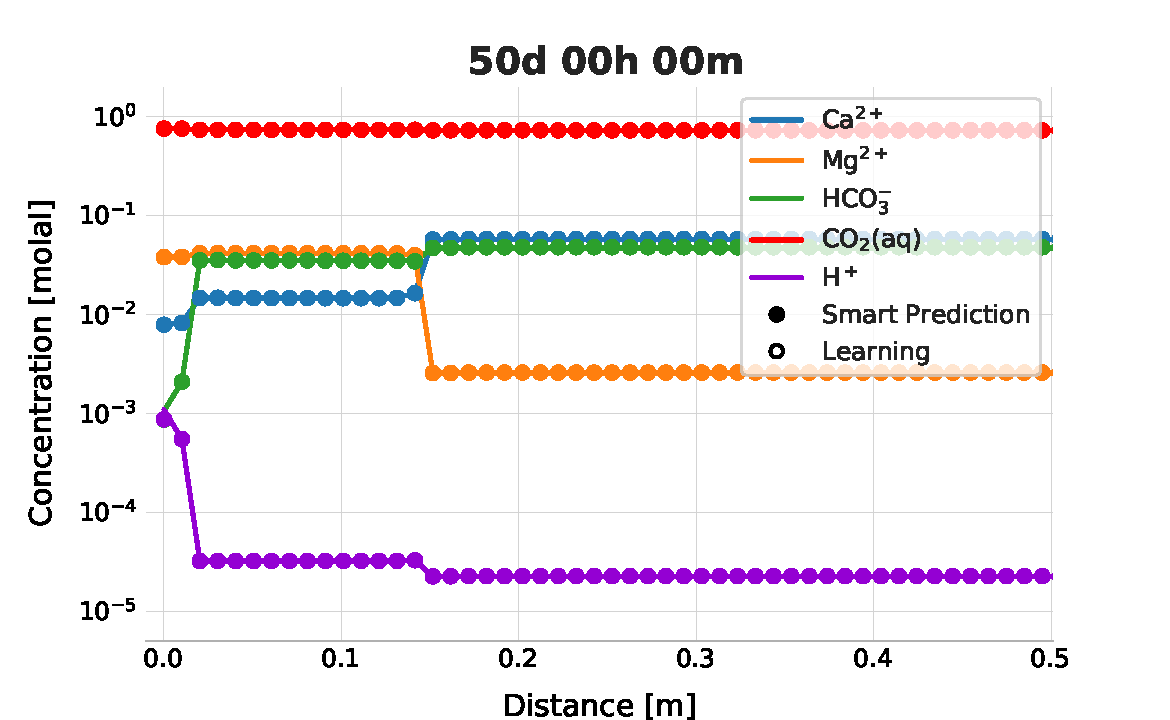
\includegraphics[width=1\textwidth]{figures/aqueous-species-2400}
\par\end{center}%
\end{minipage}
\par\end{centering}
\caption{\label{fig:calcite-dolomite}The volume percent ($\%_{\text{vol}}$)
of minerals calcite and dolomite along the rock core as well as the
concentrations of selected aqueous species (in molal) at three different
times: 30 minutes, 5 hours, and 50 days (after 1, 10, and 2400 time
steps of 30 minutes each, respectively). The \emph{solid curves} correspond
to results of the reactive transport simulation using conventional
chemical equilibrium calculations based on the Gibbs energy minimization.
The circles $\text{(}\bullet\text{)}$ and $\text{(}\circ\text{)}$
correspond to the results using smart chemical equilibrium calculations.
\emph{Solid circles} $\text{(}\bullet\text{)}$ indicate successful
fast and accurate smart equilibrium prediction at that point, whereas
the \emph{empty circles} $\text{(}\circ\text{)}$ depict the cells
where \emph{on-demand learning} was needed.}
\end{figure}


\subsection{Smart Prediction Analysis\label{subsec:Performance-and-Accuracy}}

Figure~\ref{fig:calcite-dolomite} shows the volume of minerals calcite,
CaCO$_{3}$, and dolomite, CaMg(CO$_{3}$)$_{2}$ (left), as well
as the concentrations of aqueous species Ca$^{2+}$(aq), Mg$^{2+}$(aq),
HCO$_{3}^{-}$(aq), CO$_{2}$(aq), and H$^{+}$(aq) (right) along
the rock core at three different simulation times: 30 minutes, 5 hours,
and 50 days. As calcite dissolves, Ca$^{2+}$(aq) ions are released
into the aqueous solution, which reacts with the incoming Mg$^{2+}$(aq)
ions from the left boundary to precipitate dolomite. After 30 minutes
of injecting the CO$_{2}$-saturated brine (i.e., after a single time
step), one observes a slight dissolution of calcite and corresponding
precipitation of dolomite. The injected CO$_{2}$-saturated brine
increases the local concentrations of carbonic species, CO$_{2}$(aq)
and HCO$_{3}^{-}$(aq). The local concentrations of ions Ca$^{2+}$(aq)
increases as a result of CaCO$_{3}$ dissolution. The precipitated
dolomite, however, is gradually dissolved, as the injection of the
acidic CO$_{2}$-saturated fluid continues. This can be seen in Figure~\ref{fig:calcite-dolomite}
(bottom, left), in the very left region of the rock core, where neither
calcite nor dolomite are present after 50 days of continuous fluid
injection. At the same time, after 50 days of fluid injection (i.e.,
after 2400 time steps), the Mg$^{2+}$(aq) concentration drops sharply
between core distances 0.1~m and 0.2~m, which is exactly where dolomite
is currently precipitating. Moreover, in the same region Ca$^{2+}$(aq)
concentration locally jumps as calcite dissolves.

\begin{figure}
\begin{centering}
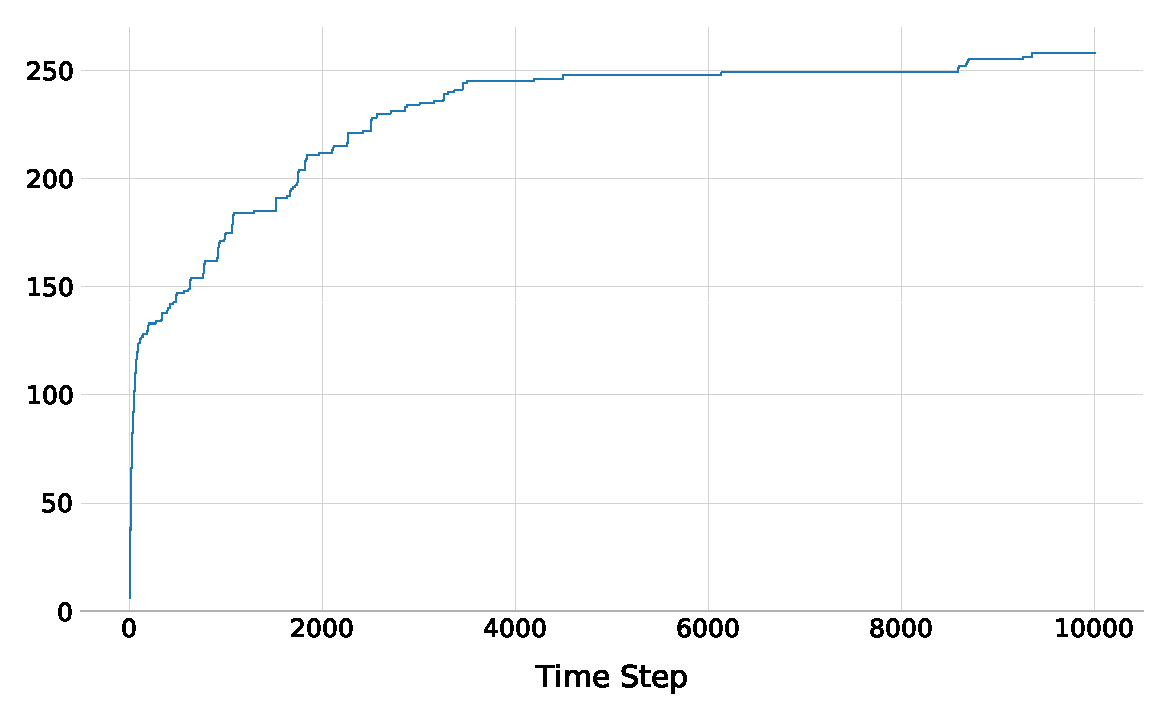
\includegraphics[width=0.7\textwidth]{figures/on-demand-learning-total}
\par\end{centering}
\caption{\label{fig:number-training-1}The accumulated number of \emph{on-demand
learning} operations triggered by the smart chemical equilibrium algorithm
during the reactive transport simulation using a mesh with 100 cells.
The simulation finished after 10'000 time steps and required thus
the solution of 1'000'000 chemical equilibrium problems. Only 258
(or 0.03\%) of these were solved using the full Gibbs energy minimization
calculation; the majority (99.97\%) were quickly and accurately estimated
with the smart chemical equilibrium algorithm.}
\end{figure}

Observe in Figure~\ref{fig:calcite-dolomite} that the use of the
smart chemical equilibrium algorithm \emph{does not} compromise accuracy
during the simulation. In this figure, the solid circles $\text{(}\bullet\text{)}$
represent a successful smart prediction of an accurate equilibrium
state at that cell position and time step, whereas the empty circles
$\text{(}\circ\text{)}$ represent a failure in this respect. The
latter happens because of the absence of a previously solved chemical
equilibrium problem similar enough to the new one. The empty circles
$\text{(}\circ\text{)}$ also denote cells at which an on-demand learning
operation was triggered, resulting in a Gibbs energy minimization
calculation (that would be needed anyway if the smart equilibrium
algorithm was not used). These on-demand learning operations are triggered
in different mesh cells, either on the same or different time steps.
We remark that the current implementation of the algorithm does not
rely on any spatial or temporal information, although this could be
explored for faster search operations in the future.

From Figure~\ref{fig:calcite-dolomite}, we also can see that during
the first time step of the simulation (30 minutes) the smart equilibrium
algorithm was able to accurately estimate the equilibrium states in
most mesh cells (see the solid circles $\bullet$). It learned enough
distinct chemical equilibrium problems on a few upstream cells (near
the left boundary) which could be successfully used for quick and
accurate estimates for the rest of the cells downstream. To be precise,
injecting the reactive fluid inside the rock core promotes strong
compositional changes in both resident fluid and rock minerals. Because
of this, during the first time step, the algorithm requires \emph{on-demand
learning} in 6 cells next to the left boundary (see the empty circles
$\circ$ in Figure~\ref{fig:calcite-dolomite}). As the perturbation
fronts move down the rock core, additional learning is performed as
needed to fulfil a given accuracy criterion; here $\epsilon_{\text{rel}}=0.1$
and $\epsilon_{\text{abs}}=10^{-8}$ are used in equation~(\ref{eq:acceptance-test-mu}).
As seen in Figure~\ref{fig:calcite-dolomite} (after 5h, or 10 time
steps), 2 cells require a full and expensive chemical equilibrium
calculation for both accuracy and on-demand learning purposes.

\begin{figure}
\begin{centering}
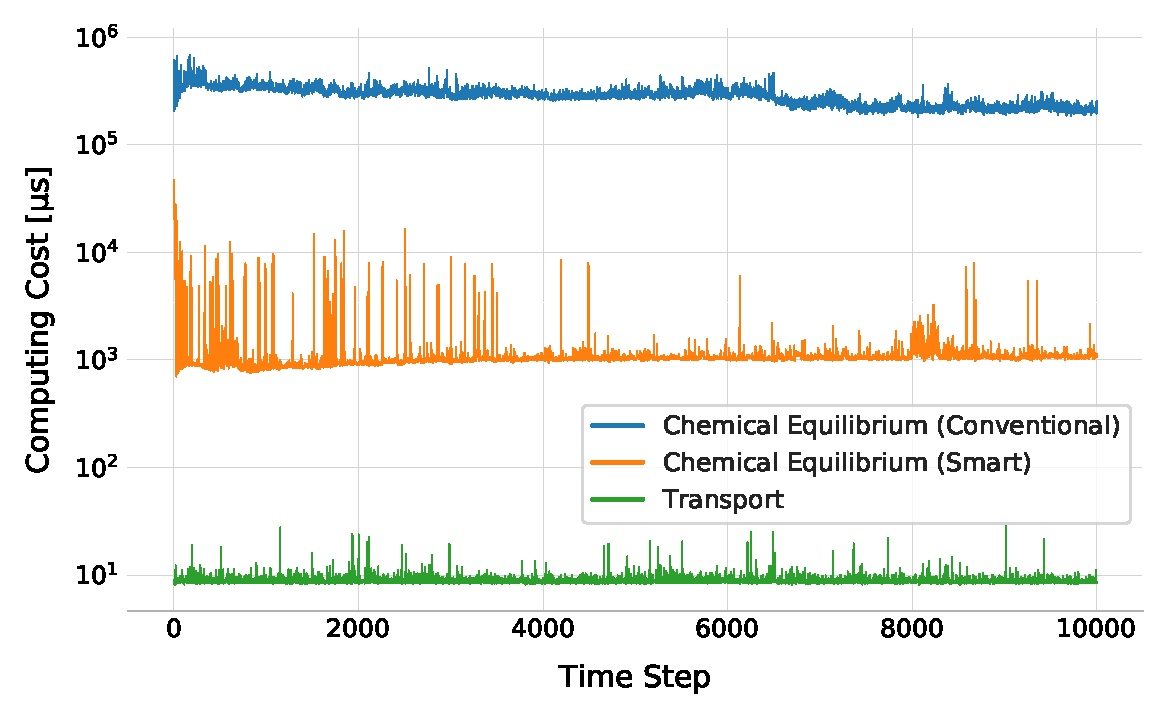
\includegraphics[width=0.7\textwidth]{figures/computing-costs}
\par\end{centering}
\caption{\label{fig:computational-cost}Comparison of the computing costs (CPU
time in microseconds) of transport, conventional, and smart chemical
equilibrium calculations during each time step of the reactive transport
simulation. The cost of equilibrium calculations per time step is
the sum of the individual costs in each mesh cell, whereas the cost
of transport calculations per time step is the time required when
solving the discretized algebraic transport equations.}
\end{figure}

Figure~\ref{fig:number-training-1} presents the number of on-demand
learning operations during the reactive transport simulation. Note
a steep growth on the initial time steps, where the smart chemical
equilibrium algorithm is very actively learning new equilibrium problems.
These are a result of the incoming brine perturbing the fluid composition
on the left side of the rock core. As time passes, the increment of
such on-demand learning operations becomes very small, about 1 or
2 cells per time step. Eventually, the smart prediction algorithm
becomes knowledgeable enough about the recurring equilibrium states
in the simulation that it can quickly and accurately perform all subsequent
equilibrium calculations without further learning or just some occasional
ones. We remark that this result is specific to the reactive transport
example investigated here. In a reactive transport problem with more
heterogeneous features, for example, one could expect more on-demand
learning operations. We plan to investigate this in future work.

Figure~\ref{fig:computational-cost} compares the computational cost,
at each time step, of: \emph{(i)} conventional chemical equilibrium
calculations, \emph{(ii)} smart chemical equilibrium calculations,
and \emph{(iii)} transport calculations. These costs are measured
as CPU time in microseconds. For the equilibrium calculations, conventional
and smart, we show CPU time needed to calculate all equilibrium states
across all mesh cells within the same time step. For the transport
calculations, the cost is the time needed to solve the algebraic transport
equations (e.g., solving sparse linear systems). Figure~\ref{fig:computational-cost}
confirms that the cost of conventional chemical equilibrium calculations
can be orders of magnitude higher than the cost of transport calculations
(five orders of magnitude higher in this relatively simple reactive
transport example). It also shows that the computational cost associated
with chemical equilibrium calculations is drastically reduced with
the smart equilibrium algorithm (by about three orders of magnitude
when smart predictions are made in all mesh cells during a time step).
Note that on the first time steps of the reactive transport simulation,
CPU cost of smart equilibrium algorithm has relatively high spikes
in comparison to those after 4000 time steps. We observe in most of
those spikes the need of on-demand learning in 1 to 2 cells (out of
100). After about half of the simulation time, the orange curve has
only sparse peaks, which corresponds to only occasional learnings
demanded by the acceptance test of the algorithm.

\begin{figure}
\begin{centering}
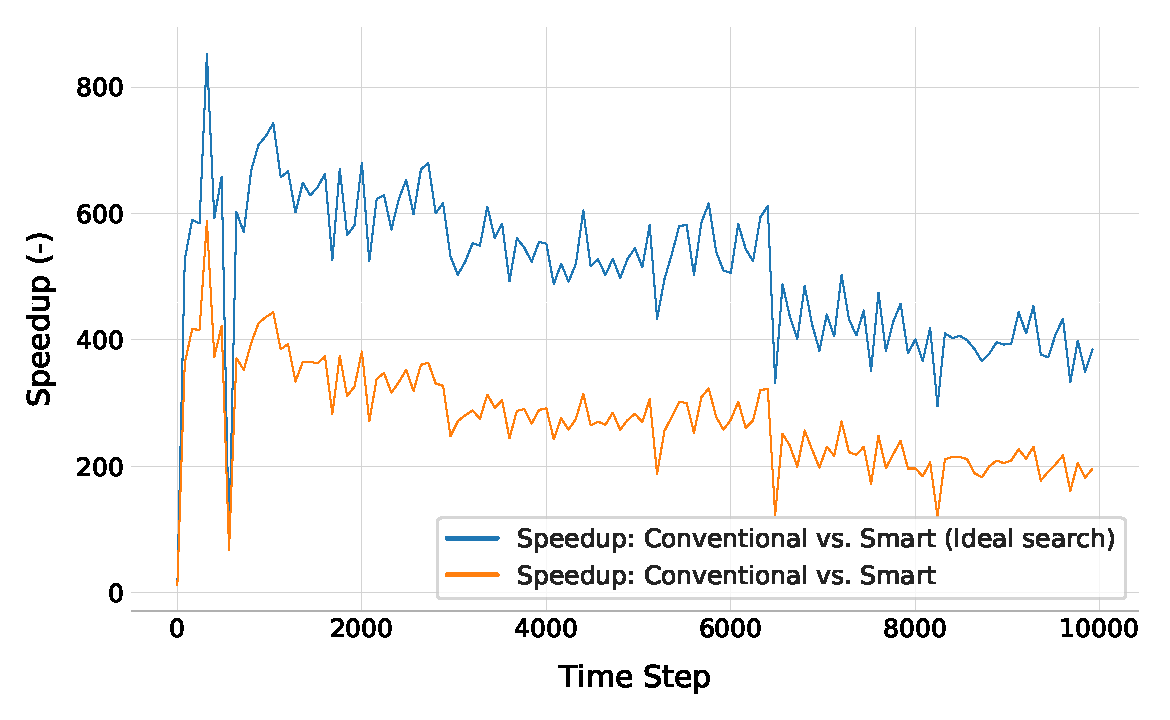
\includegraphics[width=0.7\textwidth]{figures/speedups}
\par\end{centering}
\caption{\label{fig:speedup-with-and-without-search-costs}The speedup of chemical
equilibrium calculations, at each time step of the simulation, resulting
from the use of the on-demand learning acceleration strategy (orange).
A comparison is made with the speedup obtained by removing the computing
time needed for the nearest neighbor search (blue). The latter indicates
an upper-bound for the speedup as our search algorithm is improved.}
\end{figure}


\subsection{Nearest Neighbor Search Analysis\label{subsec:Nearest-Neighbor-Search-Analysis}}

Recall that estimating an equilibrium state in a smart chemical equilibrium
calculation requires a nearest neighbor search operation. This search
is performed among all currently recorded fully solved chemical equilibrium
problems, during the ongoing reactive transport simulation. It is
needed to find the previously solved equilibrium problem whose input
conditions are the closest (in the sense of Euclidean norm) to the
input conditions of the new problem. Thus, the computing cost of the
search operation increases as we perform more on-demand learning calculations
because, at the end of these, we store a newly learned equilibrium
state.

Figure~\ref{fig:search-traylor-vs-total-learnings} demonstrates
this increase in search cost as more learned equilibrium problems
are recorded during the reactive transport simulation. It also compares
it with the cost of performing a first-order Taylor extrapolation
calculation (a small and fast matrix-vector multiplication), which
has a rather constant computing cost. This increase in search time
eventually ceases because the smart algorithm has already learned
enough key chemical equilibrium problems to quickly estimate most
(in some cases all) of the subsequent ones. However, should we have
more geologic and geochemical complexity in the simulation, this cost
could continue increasing. This most certainly implies the importance
of the switch from a linear search algorithm to a kd-tree-based nearest
neighbor search algorithm to maintain this cost constant and amenable.
Previously stored learned problems could be ranked so that those that
have not had much use for quickly predicting new states are removed
from the database. In this way the cost of the search will remain
negligible compared to other costs in the simulation.

\begin{figure}
\begin{centering}
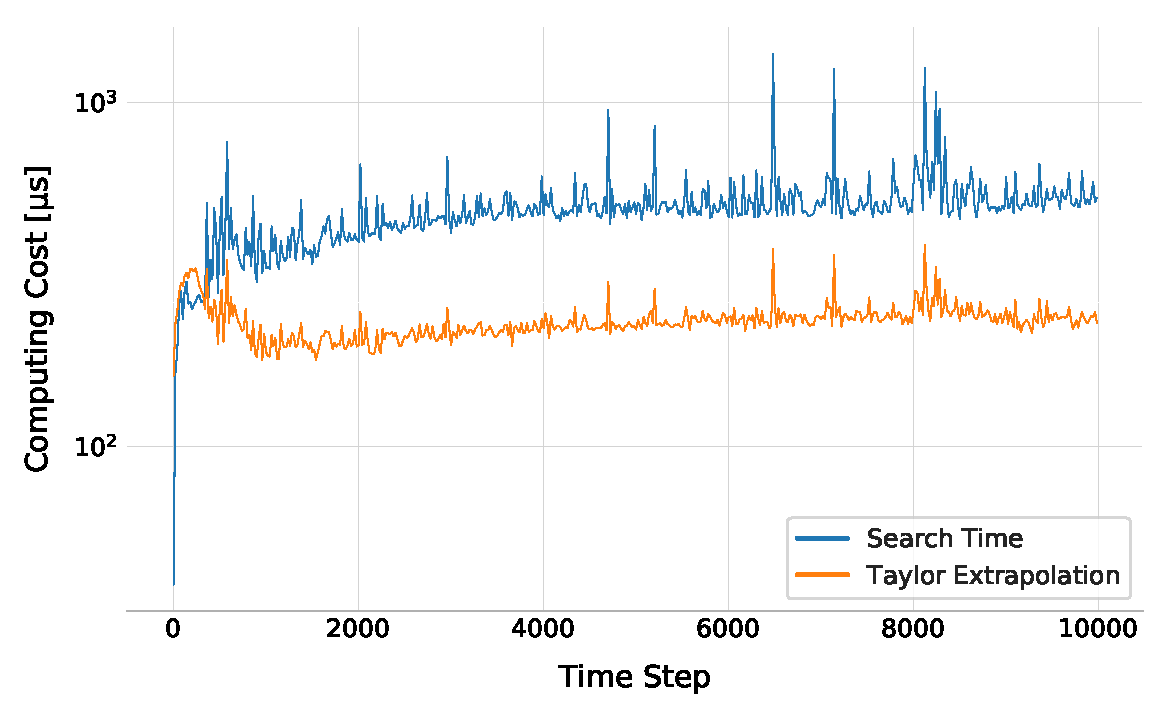
\includegraphics[width=0.7\textwidth]{figures/search-traylor-vs-total-learnings}
\par\end{centering}
\caption{\label{fig:search-traylor-vs-total-learnings}The computing time for
the nearest neighbor search operations as more fully solved equilibrium
problems are stored during the simulation. A comparison is made against
the computing time required for the first-order Taylor extrapolation
calculation, which is a small and fast matrix-vector multiplication
with more or less constant cost throughout.}
\end{figure}

Consider a \emph{hypothetical ideal nearest neighbor search algorithm}
whose computing cost is zero. We have shown that search operations
contribute to most of the cost in the smart chemical equilibrium method
because the Taylor extrapolation calculation is fast. The use of such
ideal nearest neighbor search algorithm should then give us an approximation
for the upper bound in the speedup we could ever obtain. This is shown
in Figure~\ref{fig:speedup-with-and-without-search-costs}, where
the speedup\footnote{The speedup at each time step of the reactive transport simulation
is calculated as the ratio of the accumulated time needed for the
conventional and smart chemical equilibrium calculations across all
cells in the mesh.} of our current implementation of the smart chemical equilibrium algorithm
stabilizes at a value close to 200, whereas the ideal speedup is about
400. Thus, further research and improvement in this regard is needed
for even higher efficiency. 

\section{Discussion and Conclusions\label{sec:Discussion-and-Conclusions}}

We use a smart chemical equilibrium algorithm with on-demand learning
acceleration capabilities to substantially speedup reactive transport
simulations. For the specific problem investigated in this work, we
obtain a speedup of 200 compared to the use of a conventional chemical
equilibrium algorithm. We note that this speedup is specific to the
problem studied and the assumptions made about the chemical system.
In our particular case, it consists of 36 species in total, with the
non-ideal thermodynamic behavior of the aqueous phase modeled using
the relatively expensive Pitzer model.

This substantial speedup is due to the capability of the smart chemical
equilibrium algorithm to learn previous calculations during the reactive
transport simulation. This permits thus a quick and accurate prediction
of subsequent calculations with similar input conditions (without
requiring iterative computations such as found in Newton method).
The use of sensitivity derivatives is essential for this quick estimation.
They are calculated at the end of each on-demand learning operation,
using automatic differentiation powered by \texttt{\href{http://autodiff.github.io}{autodiff}}
\citep{autodiff2018}. The estimation is carried out by means of a
first-order Taylor extrapolation, using a previously learned equilibrium
state as a reference point. This reference equilibrium state is searched
for by comparing the given input conditions for the new equilibrium
problem with the input conditions of previously solved problems in
the course of the reactive transport simulation (using the nearest
neighbor search).

We remark that the use of an on-demand learning strategy has advantages
compared to more classic machine learning algorithms. In particular,
there is no need for an \emph{a priori training stage}, which can
impose many difficulties to modelers (who should not necessarily need
to understand how algorithms work, but rather what they can solve)
and a break in their usual workflow. For modeling scenarios in which
it is not possible to have a reasonable insight of all possible geochemical
conditions the chemical system may undergo during the simulation,
a priori training can be very challenging. It can also require a comprehensive
training stage, generating extremely big data, most of which might
not even be needed. Moreover, a minimal change in modeling parameters
or configuration details is enough to make that big data obsolete
(e.g., a change of activity model, addition\slash removal of phases\slash species\slash reactions,
etc.), which can potentially compromise an exploratory modeling exercise
with many tested and analyzed setups. Last, but not the least, traditional,
statistically-based machine learning algorithms applied to chemical
equilibrium calculations neither understand the thermodynamic behavior
of stable phases nor it can straightforwardly predict equilibrium
states that satisfy mass conservation of chemical elements and electric
charges.

We plan to assess the efficiency of the smart chemical equilibrium
algorithm under more complex geochemical and geological conditions.
This includes, for example, modeling radionuclide migration in nuclear
waste repositories, degradation processes in concrete, geothermal
energy systems, and carbon dioxide storage in geologic formations.
As future work, we also consider further improvements in the nearest
neighbor search algorithm and the use of alternative criteria when
determining whether the estimated state is accurate enough. Using
a similar on-demand learning strategy for speeding up chemical kinetics
calculations in reactive transport simulations is already an ongoing
work.

This smart chemical equilibrium algorithm has been implemented in
Reaktoro (\href{https://www.reaktoro.org}{reaktoro.org}), a unified
open-source framework for modeling chemically reactive systems.

\section*{Acknowledgments}

This research project is funded by the Swiss National Science Foundation,
the Werner Siemens Foundation, and Shell. We thank these organizations
for their financial support.

\bibliographystyle{apalike-order-by-citation}
\bibliography{library,library-svetlana}

\appendix

\section{Chemical Equilibrium Equations \label{subsec:Chemical-equilibrium-equations}}

The solution of the Gibbs energy minimization problem ~(\ref{eq:gem-problem})
needs to satisfy the following \emph{first-order optimality conditions,}
also known as \emph{Karush–Kuhn–Tucker (KKT) conditions}, for a local
minimum of the Gibbs energy function $G$ \citep{Nocedal1999,Fletcher2000}:
\begin{alignat}{2}
\mu-A^{T}y-z & =0,\\
An-b & =0,\\
n_{i}z_{i} & =0 & \qquad & (i=1,\ldots,\text{N}),\\
n_{i} & \geq0 &  & (i=1,\ldots,\text{N}),\\
z_{i} & \geq0 &  & (i=1,\ldots,\text{N}),
\end{alignat}
where $y\in\mathbb{R}^{\text{E}}$ and $z\in\mathbb{R}^{\text{N}}$
are introduced \emph{Lagrange multipliers} that need to be solved
along with the specie's amounts ${n\in\mathbb{R}^{\text{N}}}$. For
more details about these Lagrange multipliers and their interpretation
as well as for instructions on how to efficiently solve these equations,
see \citet{Leal2016a,Leal2017}.

The previous chemical equilibrium equations can be written in an \emph{extended
law of mass action} (xLMA) formulation as
\begin{alignat}{2}
\ln K-\nu(\ln a+\ln w) & =0,\\
An-b & =0,\\
n_{i}\ln w_{i} & =0 & \qquad & (i=1,\ldots,\text{N}),\\
n_{i} & \geq0 &  & (i=1,\ldots,\text{N}),\\
0<w_{i} & \leq1 &  & (i=1,\ldots,\text{N}),
\end{alignat}
following the use of the extended law of mass action equations
\begin{equation}
K_{m}=\prod_{i=1}^{\text{N}}(a_{i}w_{i})^{\nu_{mi}}.\label{eq:xlma-equations}
\end{equation}
It is associated with the M linearly independent chemical reactions
among the N chemical species in equilibrium: 
\begin{equation}
0\rightleftharpoons\sum_{i=1}^{\text{N}}\nu_{mi}\alpha_{i}\qquad(m=1,\ldots,\text{M}),
\end{equation}
where ${K\in\mathbb{R}^{\text{M}}}$ is the vector of \emph{equilibrium
constants} of the reactions, with ${K_{m}=K_{m}(T,P)}$ denoting the
equilibrium constant of the $m$th reaction, and $\nu\in\mathbb{R}^{\text{M\ensuremath{\times}N}}$
is the \emph{stoichiometric matrix} of these chemical reactions, with
$\nu_{mi}$ corresponding to the stoichiometric coefficient of the
$i$th species in the $m$th reaction. Conventionally,$\nu_{mi}$
is positive if the $i$th species is a product in the $m$th reaction,
and negative if it is a reactant. Moreover, ${w\in\mathbb{R}^{\text{N}}}$
is the vector of \emph{species stability factors} that need to be
solved along with the specie's amounts ${n\in\mathbb{R}^{\text{N}}}$.
These factors are introduced to ensure that the extended law of mass
action equations (\ref{eq:xlma-equations}) are valid even when some
species in their corresponding reactions are unstable at equilibrium
(i.e., when a species belongs to a phase that is absent from equilibrium).
When all species are stable at equilibrium, it follows that ${w_{i}=1}$
and the xLMA equations reduce to the conventional LMA equations:
\begin{equation}
K_{m}=\prod_{i=1}^{\text{N}}a_{i}^{\nu_{mi}}.
\end{equation}
The number of linearly independent chemical reactions among the N
species in equilibrium is ${\text{M}=\text{N}-\text{C}}$, where ${\text{C}=\text{rank}(A)}$,
and thus whenever the formula matrix $A$ is full rank, $\text{C}=\text{E}$
and $\text{M}=\text{N}-\text{E}$. For more information on how to
solve these equations and how they are related to the conventional
law of mass action equations, see \citet{Leal2016c,Leal2017}.

\section{Reactive Transport Equations\label{sec:Reactive-Transport-Equations}}

The fundamental mass conservation equations for both fluid and solid
species are:
\begin{alignat}{2}
\frac{\partial n_{i}^{\text{f}}}{\partial t}+\nabla\cdot(\boldsymbol{v}n_{i}^{\text{f}}-D\nabla n_{i}^{\text{f}}) & =r_{i}^{\text{f}} & \qquad & (i=1,\ldots,\text{N}^{\text{f}}),\label{eq:cons-mass-fluid-species}\\
\frac{\partial n_{i}^{\text{s}}}{\partial t} & =r_{i}^{\text{s}} &  & (i=1,\ldots,\text{N}^{\text{s}}),\label{eq:cons-mass-solid-species}
\end{alignat}
where $n_{i}^{\text{f}}$ and $n_{i}^{\text{s}}$ are the \emph{bulk
concentration} of the $i$th fluid and solid species (in mol/m$^{3}$),
respectively; $\boldsymbol{v}$ is the fluid pore velocity (in m/s);
$D$ is the diffusion coefficient of the fluid species (in m$^{2}$/s);
$r_{i}^{\text{f}}$ and $r_{i}^{\text{s}}$ are the rates of production\slash consumption
of the $i$th fluid and solid species (in mol\slash s), respectively,
due to chemical reactions; and $\text{N}^{\text{f}}$ and $\text{N}^{\text{s}}$
are the numbers of fluid and solid species, respectively. Note that
the above equations assume a single fluid phase and common diffusion
coefficients for all fluid species.

By partitioning the species as fluid and solid species, the formula
matrix $A$ can be conveniently represented as:
\begin{equation}
A=\begin{bmatrix}A^{\text{f}} & A^{\text{s}}\end{bmatrix},
\end{equation}
where $A^{\text{f}}$ and $A^{\text{s}}$ are the formula matrices
of the fluid and solid partitions (i.e., the matrices constructed
from the columns of $A$ corresponding to fluid and solid species).
The concentrations of elements in both fluid and solid partitions
$b_{j}^{\text{f}}$ and $b_{j}^{\text{s}}$ can then be calculated
from the species concentrations in the same partition using: 
\begin{alignat}{2}
b_{j}^{\text{f}} & =\sum_{i=1}^{\text{N}^{\text{f}}}A_{ji}^{\text{f}}n_{i}^{\text{f}} & \qquad & (j=1,\ldots,\text{E})\\
\shortintertext{and}b_{j}^{\text{s}} & =\sum_{i=1}^{\text{N}^{\text{s}}}A_{ji}^{\text{s}}n_{i}^{\text{s}} &  & (j=1,\ldots,\text{E}).
\end{alignat}

Recall that the rates of production of the species $r_{i}^{\text{f}}$
and $r_{i}^{\text{s}}$ are exclusively due to chemical reactions.
Let $r_{i}$ denote the rate of production\slash consumption of the
$i$th species in the system (i.e., using global index, and not a
local index within the fluid or solid partition). From the mass conservation
condition for the elements (chemical elements and electrical charge),
it follows that:
\begin{equation}
\underset{\substack{\text{rate of production}\\
\text{ of element \ensuremath{j}}
}
}{\underbrace{\sum_{i=1}^{\text{N}}A_{ji}r_{i}}}=\underset{\substack{\text{rate of production}\\
\text{ of element \ensuremath{j} in}\\
\text{the fluid partition}
}
}{\underbrace{\sum_{i=1}^{\text{N}^{\text{f}}}A_{ji}^{\text{f}}r_{i}^{\text{f}}}}+\underset{\substack{\text{rate of production}\\
\text{ of element \ensuremath{j} in}\\
\text{the solid partition}
}
}{\underbrace{\sum_{i=1}^{\text{N}^{\text{s}}}A_{ji}^{\text{s}}r_{i}^{\text{s}}}}=\quad0,
\end{equation}
which is the mathematical statement for the fact that \emph{elements
are neither created nor destroyed} during chemical reactions. We can
combine this result with equations (\ref{eq:cons-mass-fluid-species})
and (\ref{eq:cons-mass-solid-species}) to derive the following conservation
equations for the elements:
\begin{equation}
\frac{\partial b_{j}^{\text{s}}}{\partial t}+\frac{\partial b_{j}^{\text{f}}}{\partial t}+\nabla\cdot(\boldsymbol{v}b_{j}^{\text{f}}-D\nabla b_{j}^{\text{f}})=0\qquad(j=1,\ldots,\text{E}).
\end{equation}

Assume that all species, fluid and solid, are in \emph{local chemical
equilibrium everywhere, at all times}. One can then perform \emph{operator
splitting steps} to solve the fundamental mass conservation equations
(\ref{eq:cons-mass-fluid-species}) and (\ref{eq:cons-mass-solid-species})
to calculate the concentrations of the species, $n_{i}$, over time.
Let $k$ denote the current \emph{time step} and $\Delta t$ the \emph{time
step length} used in the discretization of the time derivative terms.
The operator splitting steps at the $k$th time step are:
\begin{enumerate}[wide=0.0\parindent,label=\bf{Step \arabic*)}]
\item update the concentrations of the elements in the fluid partition
using:
\[
\frac{\tilde{b}_{j}^{\text{f},k+1}-b_{j}^{\text{f},k}}{\Delta t}+\nabla\cdot(\boldsymbol{v}\tilde{b}_{j}^{\text{f},k+1}-D\nabla\tilde{b}_{j}^{\text{f},k+1})=0\qquad(j=1,\ldots,\text{E}),
\]
where $\tilde{b}_{j}^{\text{f},k}$ is the known concentration of
the $j$th element at time step $k$ in the fluid partition and $\tilde{b}_{j}^{\text{f},k+1}$
is its unknown concentration at the next time step. Note that an implicit
scheme is assumed.
\item update the total concentrations of the elements:
\begin{equation}
b_{j}^{k+1}=\tilde{b}_{j}^{\text{f},k+1}+b_{j}^{\text{s},k}.
\end{equation}
\item calculate the concentrations of the species, $n_{i}^{k+1}$, in each
mesh cell, using the full or smart chemical reaction algorithm. For
this, use the local temperature and pressure values together with
the \emph{updated local concentrations of elements}, $b_{j}^{k+1}$,
as inputs.
\end{enumerate}

\end{document}
